\chapter{Software design}

\label{ch:Software design}

\setlength{\parindent}{4em}
\setlength{\parskip}{1em}
\renewcommand{\baselinestretch}{1.5}

\section{System architecture}

In our project, we use two algorithms to stimulate the subject. First use ERPs which is different in stimulating time. Second is SSVEP which difference in stimulating frequency.

\begin{figure}[ht]
	\centering
	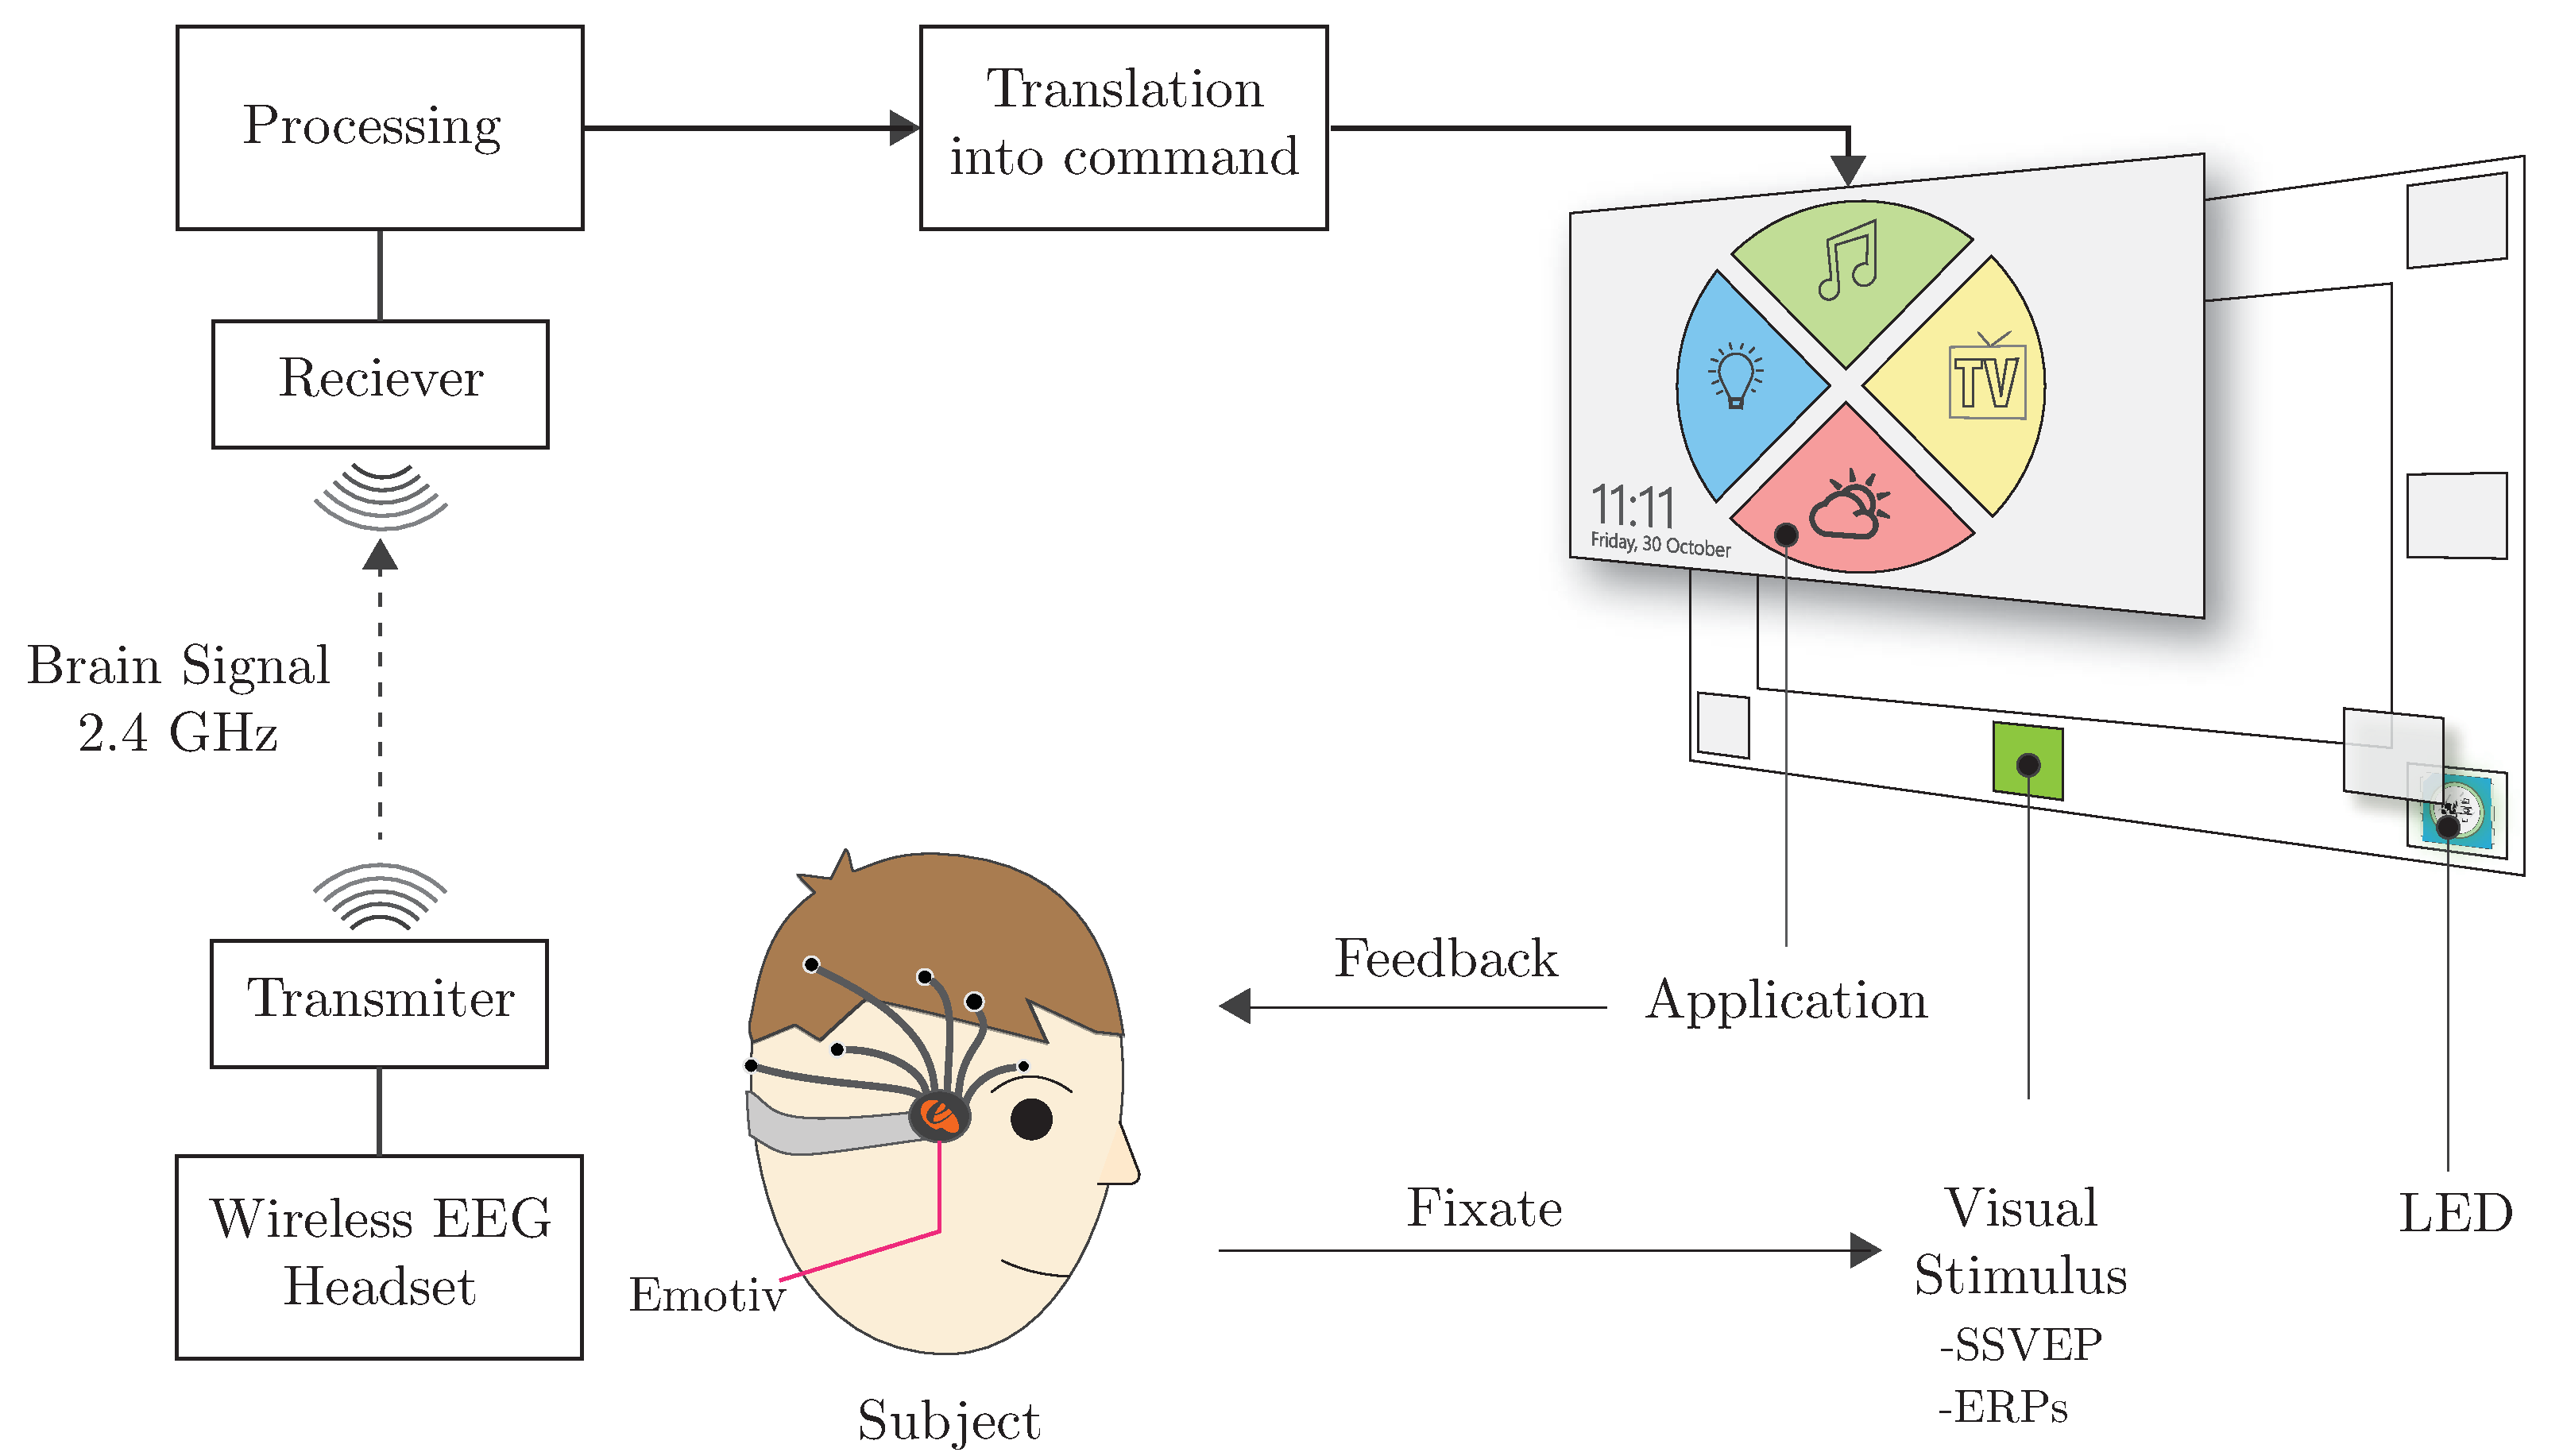
\includegraphics[scale = 0.28]{chapter5/architec.pdf}
	\caption{System architecture design}
\end{figure}

\newpage
\section{Class Diagram}

\begin{figure}[ht]
	\centering
	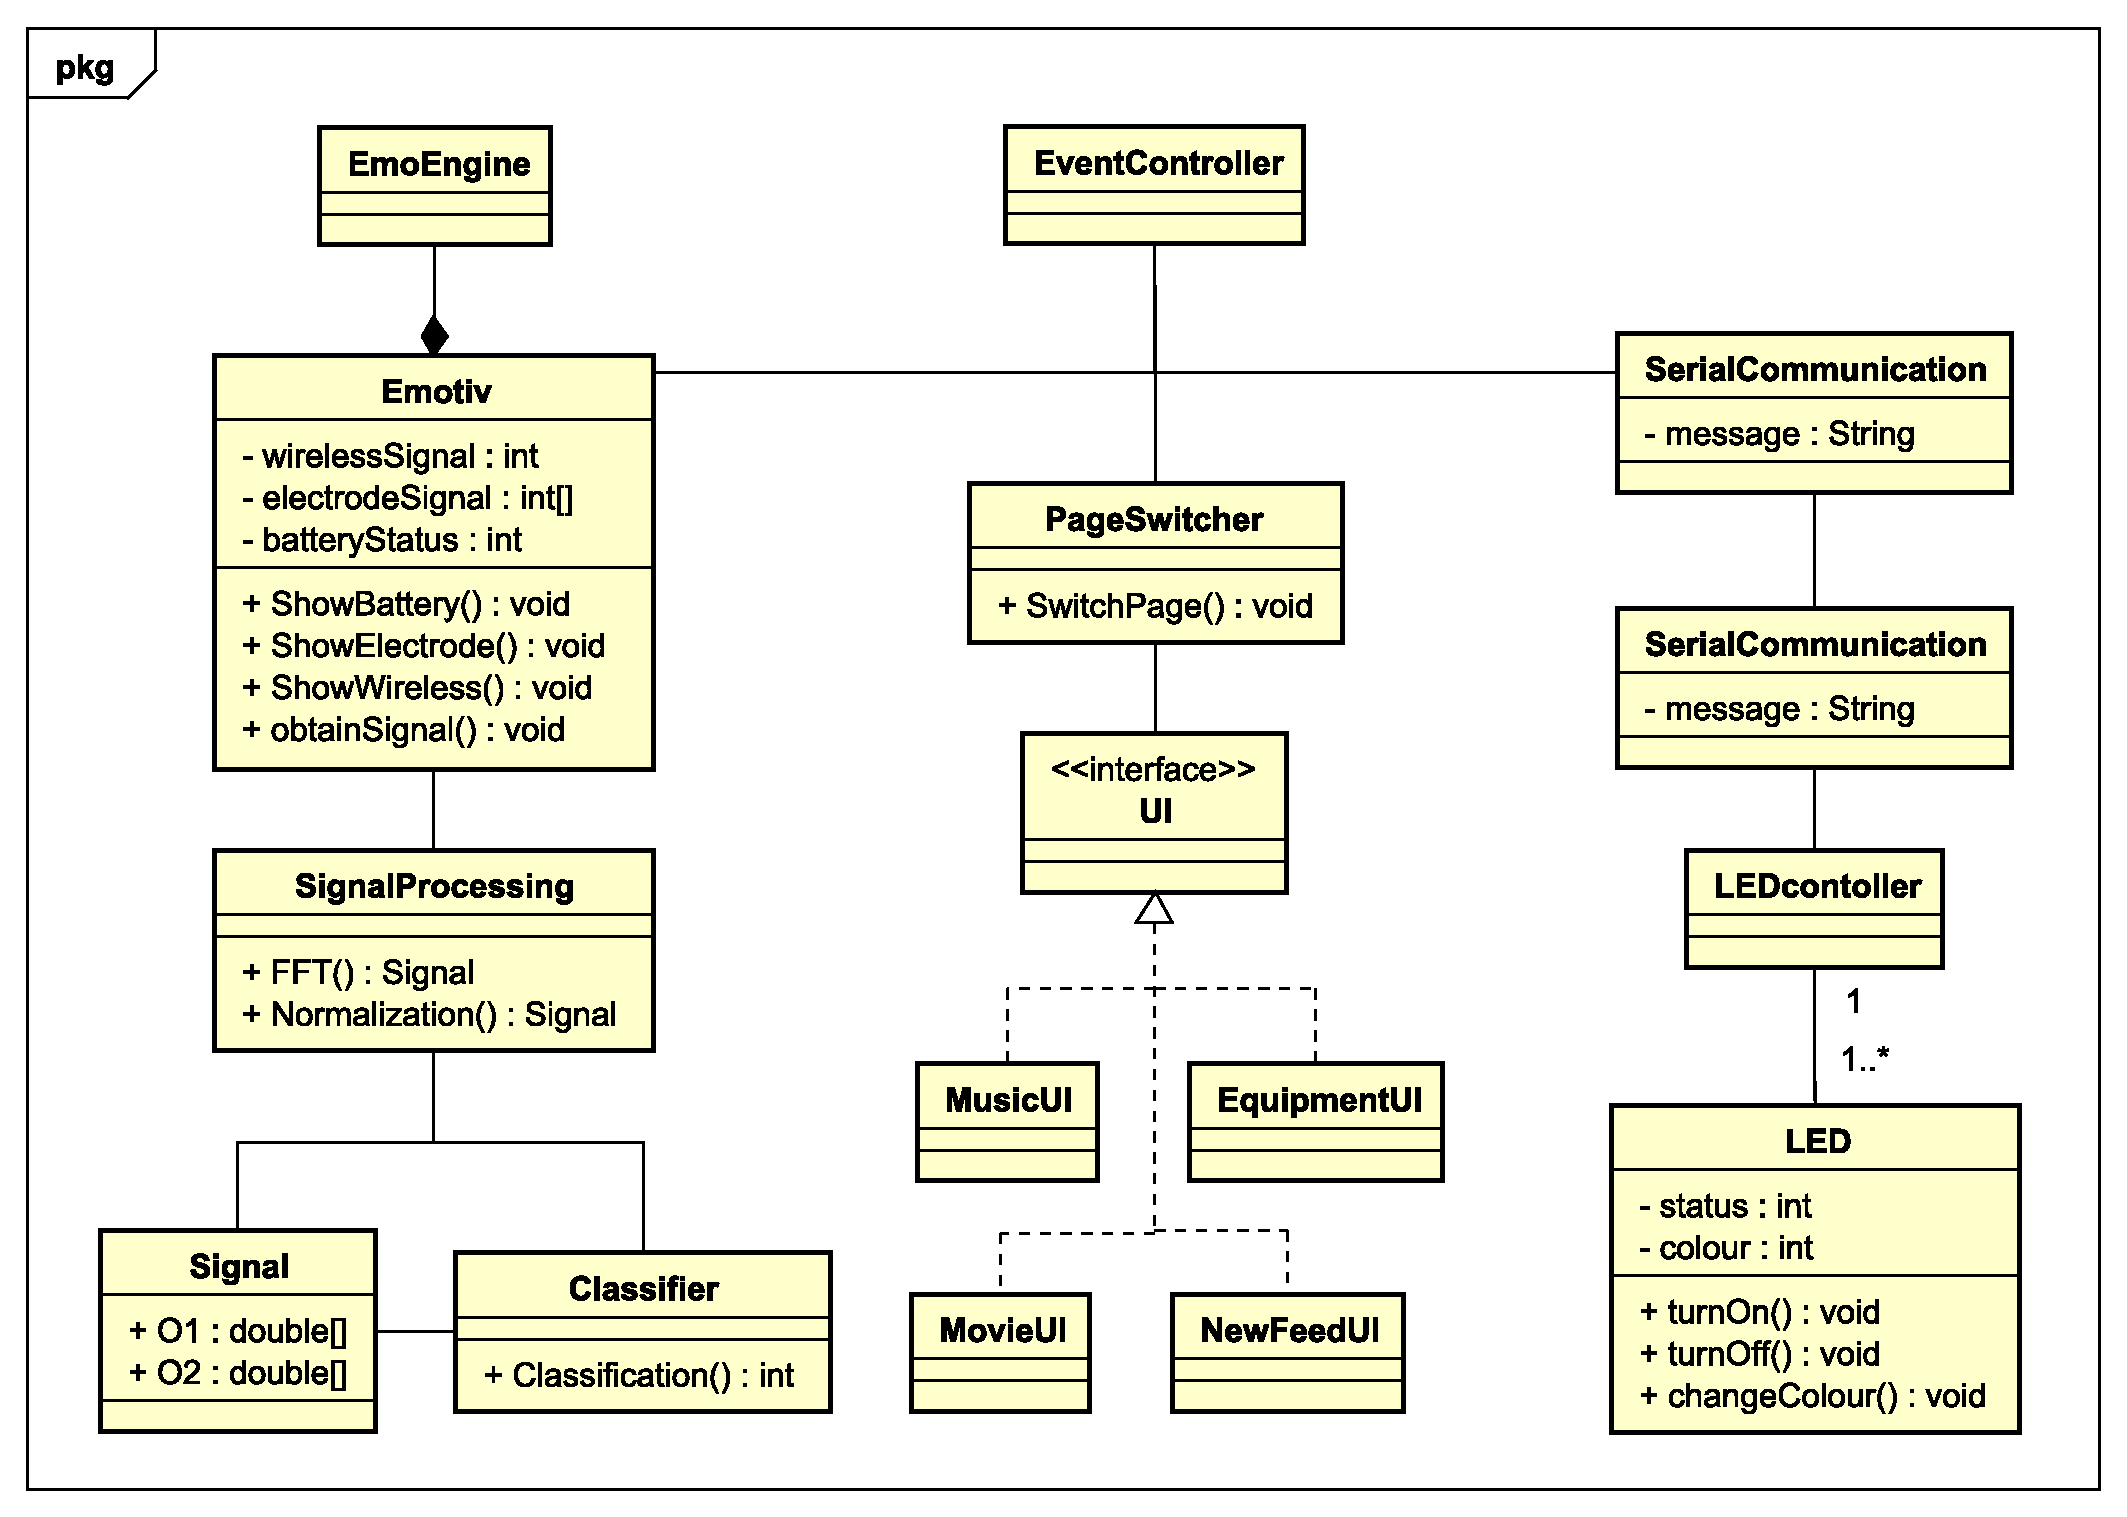
\includegraphics[scale = 0.5]{chapter5/Class.pdf}
	\caption{Class diagram}
\end{figure}

Class diagram description, starting with the most importance class, EventController, it is connecting Emotiv headset, PageSwitcher, and Serial communication classes together to make a program work in unison,

EmoEngin is a library use for connecting our program to an Emotiv headset.  Emotiv class is a substitute of a headset. it has a property of wireless signal quality, electrode contact quality, battery level which is obtained via EmoEngin. The signal class represents the EEG signal that obtains from Emotiv headset. in this project is use the only occipital channel, so the attribute is only O1 and O2. the SignalProcessing class contains an algorithm to process EEG signal to a frequency domain to perform analysis and to have standardized by normalization. the Classifier class is to classify a feature from the processed signal. the result will tell which flicker user fixate at. then it will send the result to EventController to do further step.